\graphicspath{{fig/bayes_intro/}}

\chapter{Bayesian statistics}
\label{cha:bayes_intro}

In this thesis we utilise methods from Bayesian inference to fit mathematical
models of collective behaviour to real and simulated data. Bayesian inference
represents a fully probabilistic approach to parameter inference. This allows a
practitioner to quantify their uncertainties about inferred parameter values.
In addition to this, the Bayesian framework permits flexible model structures
and potential inclusion of expert information via the prior distribution. With
this we seek to fit newly acquired data to generalisations of a popular
agent-based model from the literature.

In this chapter we shall introduce and outline some important concepts of
Bayesian inference. Algorithms to infer model parameters from data will be
presented, and the interpretation of such output shall be discussed.

\section{Bayesian inference}
\label{sec:bayesian_inference}

Having observed data $x$ we wish to quantify our beliefs about the model
parameters $\theta = (\theta_1,\theta_2,\dots,\theta_d)^T$. Given the observed
data, the likelihood function is defined as:
\begin{equation}
  L(\theta \given x) = f(x \given\theta).
\end{equation}
The likelihood represents the probability density of observing data $x$, given
the model parameters $\theta$. The prior distribution $\pi(\theta)$ is used to
quantify our prior knowledge about the parameters. Bayes' Theorem provides a
way to realise posterior beliefs from a combination of our prior beliefs and
the likelihood of the data:
\begin{equation}
  \label{eq:bayes_theorem}
  \pi(\theta \given x) =
    \frac{\pi(\theta) L(\theta\given x)}%
         {\int_{\theta} \pi(\theta) L(\theta\given x) \, \textup{d}\theta}.
\end{equation}
As the integral in the denominator is not a function of $\theta$ we may
consider it a constant of proportionality. With this we can express our
posterior beliefs as proportional to the product of the likelihood and our
prior beliefs:
\begin{align*}
  \pi(\theta\given x) & \propto \pi(\theta) \times L(\theta\given x), \\
  \text{posterior}    & \propto \text{prior} \times \text{likelihood}.
\end{align*}

\section{Markov chain Monte Carlo (MCMC)}
\label{sec:mcmc}

For the most part, the normalising constant (given in the denominator of
\cref{eq:bayes_theorem}) will have multiple dimensions, not produce a density
function of standard form, and be difficult to evaluate in all but the most
trivial cases. Markov chain Monte Carlo algorithms provide methods to sample
from the targeted density $\pi(\theta \given x)$, whilst avoiding the
evaluation of the bothersome normalising constant.

\subsection{Metropolis--Hastings}
\label{ssec:metropolis_hastings}

The Metropolis--Hastings algorithm is a popular MCMC scheme. The algorithm was
introduced by \textcite{metropolis53} in a now classic paper, and was later
generalised by \textcite{hastings70}. The algorithm works by constructing a
Markov chain which has stationary distribution equivalent to the target
distribution.

\begin{algorithm}
  \caption{Targeting $\pi(\theta \given x)$ with $n$ iterations of the
    Metropolis--Hastings algorithm.}
  \label{alg:metropolis_hastings}
  \begin{algorithmic}[1]
    \State Initialise chain with $\theta^{(0)}$
    \For{i}{1}{n}
      \State Propose ${\theta}^\star \sim q(\theta^{(i)} \given \theta^{(i-1)})$
      \State Construct acceptance probability $\alpha(\theta^\star \given \theta^{(i-1)})$ as
      \begin{equation*}
          \alpha(\theta^\star \given \theta^{(i-1)}) =
        \min\bigg\{1,
        \frac{\pi(\theta^\star) \, L(\theta^\star \given  x)}%
        {\pi(\theta^{(i-1)}) \, L(\theta^{(i-1)} \given  x)}
        \frac{q(\theta^{(i-1)} \given \theta^\star)}%
        {q(\theta^\star \given \theta^{(i-1)})}
        \bigg\}.
      \end{equation*}
      \State Draw $u \sim$ Uniform$(0, 1)$
      \If{$u \leq \alpha(\theta^\star \given \theta^{(i-1)})$}
        \State \Comment{Accept proposal}
        \State $\theta^{(i)} \leftarrow \theta^\star$
      \Else
        \State \Comment{Reject proposal}
        \State $\theta^{(i)} \leftarrow \theta^{(i-1)}$
      \EndIf
    \EndFor
  \end{algorithmic}
\end{algorithm}

The algorithm begins by initialising a Markov chain with parameters
$\theta^{(0)}$. Next, the algorithm proposes new parameter values
$\theta^\star$ from a proposal distribution $q(\theta^\star \given
\theta^{(i-1)})$. The proposed values are accepted with probability
$\alpha(\theta^\star \given \theta^{(i-1)})$. If the proposal is accepted the
next state of the Markov chain is set to the proposed value. Otherwise, the
next state is set to the current value. The acceptance probability depends on a
ratio of the posterior density evaluated at the current state and the posterior
density evaluated at the proposed state. In this ratio the normalising
constants from \cref{eq:bayes_theorem} cancel, and we see that the target
distribution need only be known up to a constant of proportionality. The
process of proposing and accepting or rejecting proposals continues until a
satisfactory number of draws are made. Metropolis--Hastings is described more
formally in \cref{alg:metropolis_hastings}.

\subsubsection{Choosing a Proposal Distribution}
\label{ssec:proposal_distribution}

The practitioner must choose a suitable proposal distribution $q(\theta^\star
\given \theta)$. Ideally the choice of proposal distribution will give rapid
convergence to $\pi(\theta \given x)$, and efficiently explore the support of
$\pi(\theta \given x)$. However, it is not obvious how a proposal distribution
should be constructed to realise these desires.

A special case of Metropolis--Hastings arises when the proposal distribution is
symmetric. Symmetric proposals have the property that:
\begin{equation*}
  q(\theta^\star \given \theta) = q(\theta \given \theta^\star).
\end{equation*}
This symmetry results in a simplification of the acceptance ratio:
\begin{equation*}
  \alpha({\theta}^\star \given \theta^{(i-1)})
    = \text{min}\,\bigg\{1,
                        \frac{\pi(\theta^\star)}{\pi(\theta^{(i-1)})}%
                        \frac{L(\theta^\star \given  x)}%
                        {L(\theta^{(i-1)} \given  x)}
                  \bigg\}.
\end{equation*}

The random walk sampler is a popular implementation of Metropolis--Hastings
which makes use of symmetric proposals. Here, proposals are generated as
\begin{equation*}
  \theta^\star = \theta^{(i-1)} +  \omega^{(i-1)},
\end{equation*}
where the $\omega$ are sampled as
\begin{equation*}
   \omega^{(i-1)} \sim \mathcal{N}_d(0, \Sigma),
\end{equation*}
and $\mathcal{N}_d$ denotes a $d$-dimensional multivariate normal distribution.
The parameter $\Sigma$ is called the `tuning parameter' and controls how the
chain moves around the parameter space.

Mixing describes how efficiently a chain moves around the sample space, and how
long it takes for the chain to converge to the target distribution. Crucially
then, the parameter $\Sigma$ can be used to control the mixing of chains. So,
naturally, we desire to select a $\Sigma$ which produces well-behaved chains.
Such a tuning parameter should allow rapid convergence to $\pi(\theta \given
x)$ and facilitate exploration of the entire support of the target. If the
target distribution is Gaussian, it has been shown that $0.234$ is an optimum
acceptance probability to try achieve \parencite{roberts01}. In an attempt to
tune $\Sigma$ to obtain an optimum acceptance probability, a common technique
is to chose 
\begin{equation*}
  \Sigma = \frac{2.38^2}{d} \widehat{\text{Var}}(\theta \given x).
\end{equation*}

However, even with strategies to try select some optimum innovation structure,
random walk samplers tend to perform poorly in high-dimensional spaces.
Consider that as the dimension of a problem increases, the probability of
proposing a point out in the tails of the target distribution increases. As a
result the acceptance probability becomes small and produces a Markov chain
which rarely moves. The acceptance probability can be increased by choosing a
$\Sigma$ which results in smaller innovations. However, this has the
consequence of producing a Markov chain which explores the sample space slowly,
and converges to the target distribution slowly.

Fortunately, there exist more sophisticated proposal mechanisms which perform
better than random walk samplers in higher dimensional problems. One such
sampler is represented by Hamiltonian Monte Carlo, which seeks to utilise
information about the gradient of the target distribution to inform
innovations. With a problem of dimension $d$, the computational expense of a
random-walk sampler is $O(d^2)$, whereas the cost of Hamiltonian Monte Carlo is
roughly $O(d^{5/4}$) \parencite{creutz88}. 

\subsection{Hamiltonian Monte Carlo (HMC)}

Hamiltonian Monte Carlo, originally Hybrid Monte Carlo, was first introduced by
\textcite{duane87}. In this now landmark paper, the HMC algorithm was detailed
and used for numerical simulation of Lattice Quantum Chromodynamics. Following
this, Radford Neal recognised the potential statistical applications of HMC,
and used it in his work on Bayesian neural network models \parencite{neal95}.
However, it wasn't really until Neal's 2011 review \parencite{neal11} that HMC
received mainstream attention in statistical computing
\parencite{betancourt18}.

Hamiltonian Monte Carlo is a realisation of the Metropolis--Hastings algorithm.
Here, new parameter values are proposed by computing trajectories of motion
according to Hamiltonian dynamics. With this proposal mechanism it is possible
to propose parameter values which are distant from the current state, but which
retain a high probability of acceptance. As a result, this proposal mechanism
represents an efficient method of traversing a parameter space, and circumvents
the slow exploration of the parameter space typically experienced by random
walk samplers in higher-dimensions.

\subsubsection{Mathematical formulation}

Hamiltonian mechanics represents a reformulation of classical mechanics. In
Hamiltonian mechanics a  system is described by a $d$-dimensional position
vector, $\theta$, and a $d$-dimensional momentum vector, $p$. This system then
evolves through time according to Hamilton's equations:
\begin{align}
  \begin{split}
    \pdv{p_i}{t}      &= - \pdv{\mathcal{H}}{\theta_i},      \\
    \pdv{\theta_i}{t} &= \hphantom{-} \pdv{\mathcal{H}}{p_i},
  \end{split}
\end{align}
where $i=1,\ldots,d$ and $\mathcal{H}(\theta,  p)$ is the Hamiltonian. The
Hamiltonian is often interpreted to represent the total energy of a system,
which can be considered as the sum of the kinetic energy, $T$, and potential
energy, $V$:
\begin{equation}
  \label{eq:hamiltonian_decomp}
  \mathcal{H}(\theta, p) = T(p) + V(\theta).
\end{equation}

We wish to explore our target distribution (typically the posterior
distribution) as if evolving some Hamiltonian system. This can be achieved if
we expand our $d$-dimensional parameter space into $2d$-dimensional phase
space. Our current state can be considered as the position vector, $\theta$.
Introducing auxiliary momentum variables, $p$, expands our parameter space into
phase space, as desired.

With our parameter space extended to phase space, we must also expand our
target distribution to phase space. To do so we formulate the canonical
distribution, a joint density function over phase space:
\begin{equation}
  \label{eq:canonical_dist}
  \pi(\theta, p) = \pi(p \given\theta) \, \pi(\theta).
\end{equation}
The momentum is typically introduced as:
\begin{equation}
  p \given \theta \sim \mathcal{N}_d(0, M),
\end{equation}
where $M$ is a positive-definite ``mass matrix'', often chosen as the identity
matrix or some scalar multiple of the identity matrix. See that marginalising
out the momentum in \cref{eq:canonical_dist} recovers the target distribution.

To proceed, we consider expressing the canonical distribution as the negative
exponent of a Hamiltonian:
\begin{equation}
  \label{eq:canonical_as_hamiltonian}
  \pi(\theta, p) = \exp{-\mathcal{H}(\theta, p)}.
\end{equation}
Taking the logarithm of \cref{eq:canonical_as_hamiltonian} and using
\cref{eq:canonical_dist} we see
\begin{equation}
  \label{eq:canonical_decomp}
  \mathcal{H}(\theta, p) = -\log{\pi(p \given\theta)} - \log{\pi(\theta)}.
\end{equation}
Recall from \cref{eq:hamiltonian_decomp} that the total energy in a system can
be considered as the sum of the system's kinetic energy and potential energy.
If we compare \cref{eq:hamiltonian_decomp} and \cref{eq:canonical_decomp} we
can see that we have constructed a system with kinetic energy given by the
negative logarithm of the momentum density, and potential energy given by the
negative logarithm of the target density, that is:
\begin{equation*}
    T(p) = -\log{\pi(p \given\theta)} \quad\text{and}\quad V(\theta) = -\log{\pi(\theta)}.
\end{equation*}

\subsubsection{Computer implementation, NUTS \& Stan}

Now that we have described HMC we are in a position to consider its
implementation \emph{in silico}. For computer implementation we must first be
able to approximate solutions to Hamilton's equations. Such approximations can
be achieved by discretising time using some small time step $\epsilon$. Next,
the practitioner must also choose the number of steps $L$ for which to simulate
Hamilton's equations. With this in place, the practitioner typically implements
the leapfrog method to solve Hamilton's equations \parencite{neal11}.
\cref{alg:hmc} details a realisation of HMC in practice, and demonstrates the
leapfrog method to simulate Hamiltonian mechanics.

\begin{algorithm}[tb]
  \caption{Targeting $\pi(\theta \given x)$ with $n$ iterations of Hamiltonian Monte
  Carlo, using $L$ steps and discretisation $\epsilon$.}
  \label{alg:hmc}
  \begin{algorithmic}[1]
    \State Initialise chain with $\theta^{(0)}$
    \For{i}{1}{n}
      \State Draw momentum $p^{(i-1)} \sim \mathcal{N}_d(0, M)$
      \State $p^\star \leftarrow p^{(i-1)}$
      \State $\theta^\star \leftarrow\theta^{(i-1)}$
      \State \Comment{Simulate Hamiltonian with leapfrog method for $L$ steps and 
      discretisation $\epsilon$}
      \For{j}{1}{L}
        \State $\theta^\star$, $p^\star \leftarrow$ Leapfrog$(\theta^\star$,
                                                             $p^\star$, $\epsilon)$
      \EndFor
      \State Construct acceptance probability $\alpha(\theta^\star, p^\star \given
                                               \theta^{(i-1)}, p^{(i-1)})$ as
        \begin{equation*}
            \alpha(\theta^\star, p^\star \given\theta^{(i-1)}, p^{(i-1)}) =
            \min\big\{1, \exp[\mathcal{H}(\theta^{(i-1)}, p^{(i-1)}) -
                              \mathcal{H}(\theta^\star, p^\star)]
                  \big\}
        \end{equation*}
      \State Draw $u \sim$ Uniform$(0, 1)$
      \If{$u \leq \alpha(\theta^\star, p^\star \given\theta^{(i-1)}, p^{(i-1)})$}
        \State \Comment{Accept proposal}
        \State $\theta^{(i)} \leftarrow\theta^\star$
      \Else
        \State \Comment{Reject proposal}
        \State $\theta^{(i)} \leftarrow\theta^{(i-1)}$
      \EndIf
    \EndFor
  \State
  \Procedure{Leapfrog}{$\theta$, $p$, $\epsilon$}
    \State $p \leftarrow p + \frac{\epsilon}{2} \pdv{V}{\theta}$
    \State $\theta \leftarrow \theta + \epsilon M^{-1} p$
    \State $p \leftarrow p + \frac{\epsilon}{2} \pdv{V}{\theta}$
    \State \Return $\theta$, $p$
  \EndProcedure
  \end{algorithmic}
\end{algorithm}

As we have seen, in implementing HMC it is left to the practitioner to choose
appropriate values for the number of steps $L$, the step size $\epsilon$, and
the mass matrix $M$. Unfortunately, making a poor choice for any of these
parameters can result in a significant decrease in the performance of HMC
\parencite{hoffman14}. Fortunately, $\epsilon$ can be tuned during the
algorithm's implementation, using ideas from the adaptive MCMC literature.
However, there is no easy way to select a value of $L$ \emph{a priori}.
Typically, a practitioner will have to make multiple costly tuning runs in
order to select an appropriate value of $L$.

It was with this tuning problem in mind that \textcite{hoffman14} introduced
the No-U-Turn Sampler (NUTS). This algorithm extends HMC and eliminates the
need for the parameter $L$. Using ideas from stochastic optimisation in
numerical analysis, the authors were able to tune $\epsilon$ and $M$ during the
implementation of their algorithm. NUTS performs \emph{at least} as efficiently
as, and often \emph{more} efficiently than, an equivalent well-tuned
implementation of a standard HMC method. Altogether then, NUTS represents an
efficient implementation of a HMC-like algorithm, where the practitioner is
left free of the obligation of choosing any tuning parameters. 

Although NUTS relieves the practitioner the obligation of selecting parameters
$\epsilon$ and $L$, its implementation remains far from trivial. Here enters
Stan. Stan, named after Stanislaw Ulam, one of the original pioneers of Monte
Carlo methods \parencite{metropolis49}, is a probabilistic programming language
implemented in C++ \parencite{gelman15}. Stan requires the user to construct a
Stan program, which specifies how to compute the log-posterior density for
their model of interest \parencite{stanteam15}. With this, Stan implements the
NUTS algorithm, and returns to the user samples from the desired posterior
density.

\subsection{Convergence diagnostics}
\label{ssec:convergence_diagnostics}

Although there exist empirical methods which seek to assess convergence of
chains, it is also appealing to analyse the output of our schemes in an attempt
to inspect convergence. One of the simplest informal methods to assess
convergence is to inspect the trace plots of a scheme and check for any
irregularities. For a more robust inspection of convergence it is advisable to
run multiple chains initialised at different locations
(\cref{fig:convergence}).
\begin{figure}[tb]
  \begin{subfigure}[b]{0.5\textwidth}
    \centering
    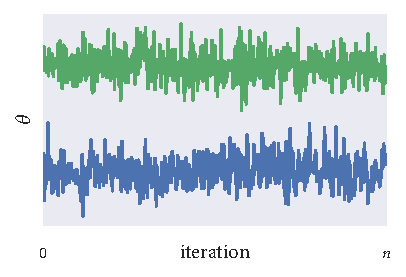
\includegraphics{B.pdf}
    \subcaption{}
    \label{fig:B}
  \end{subfigure}%
  \begin{subfigure}[b]{0.5\textwidth}
    \centering
    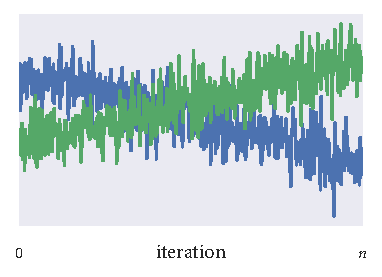
\includegraphics{W.pdf}
    \subcaption{}
    \label{fig:W}
  \end{subfigure}
  \caption{The importance of running multiple chains. \subref{fig:B} If only a
    single chain had been inspected, here we may have concluded that the
    corresponding sampler had converged. However, in running multiple chains
    it is clear that the chains have \emph{not} converged to a common
    distribution. \subref{fig:W} Likewise, viewed separately, the trajectories
    here do not appear stationary, but taken together they do appear to cover a
    common distribution.}
  \label{fig:convergence}
\end{figure}

\subsubsection{Split-$\widehat{R}$}

Split-$\widehat{R}$ represents a popular convergence diagnostic
\parencite{gelman13}. This measure uses information about the within-chain
variance \emph{and} between-chain variance to quantify how well chains have
mixed.

Consider that we have $m$ chains of length $n$, which target some estimand of
interest $\theta$. We label the draws as $\theta^{(i, j)}$ for $i=1,\ldots,n;
j=1,\ldots,m$. The between-chain variance $B$ is then computed as:
\begin{equation*}
  B = \frac{n}{m - 1} \sum_{j=1}^m (\bar{\theta}^{(\cdot, j)} - \bar{\theta}^{(\cdot,\cdot)})^2
    \quad \text{where} \quad
    \bar{\theta}^{(\cdot, j)} = \frac{1}{n} \sum_{i=1}^{n} \theta^{(i, j)},
    \quad
    \bar{\theta}^{(\cdot, \cdot)} = \frac{1}{m} \sum_{j=1}^m \bar{\theta}^{(\cdot, j)}.
\end{equation*}
The within-chain variance $W$ is captured in a similar manner:
\begin{equation*}
  W = \frac{1}{m} \sum_{j=1}^m s_j^2,
    \quad \text{and} \quad
    s_j^2 = \frac{1}{n-1} \sum_{i=1}^{n}(\theta^{(i, j)} - \bar{\theta}^{(\cdot,j)})^2,
\end{equation*}
The between-chain and within-chain variance can be combined in a weighted sum
to estimate the marginal posterior variance of the estimand:
\begin{equation}
  \label{eq:marg_post_var}
  \widehat{\text{Var}}^+ (\theta \given x) = \frac{n-1}{n} W + \frac{1}{n} B.
\end{equation}
The convergence diagnostic split-$\widehat{R}$ is then computed as:
\begin{equation}
  \label{eq:rhat}
  \widehat{R} = \sqrt{\frac{\widehat{\text{Var}}^+ (\theta \given x)}{W}}.
\end{equation}
From \cref{eq:marg_post_var} observe that as $n\rightarrow\infty$ the estimated
marginal posterior variance tends to $W$. With this, and \cref{eq:rhat}, we see
that $\widehat{R}\rightarrow1$ as $n\rightarrow\infty$. As such, we look to
compute $\widehat{R}\approx1$ to indicate that a sampler has converged.

\subsubsection{Effective sample size}

The effective sample size is introduced as a notion to assess the `size' of a
sample when the samples are correlated. The idea is that $10,000$
autocorrelated samples from a distribution represent less information than
$10,000$ \emph{independent} samples from that same distribution. The effective
sample size can be considered to penalise sample size by the autocorrelation of
the draws.

For a single chain, a common definition of the effective sample size is:
\begin{equation}
    \label{eq:ess}
    \text{ESS} = \frac{n}{1 + 2 \sum_{k=1}^\infty \rho_k},
\end{equation}
where $n$ is the number of samples and $\rho_k$ is the autocorrelation at lag
$k$. Although a popular definition, in practice this measure is often too
optimistic when chains haven't converged. The practitioner must also decide
when to truncate the infinite sum which appears in the denominator.

A more sophisticated estimate of the effective sample size is presented by
\textcite{gelman13}. In this definition the authors circumvent the infinite sum
in the denominator of \cref{eq:ess}. The inclusion of between-chain variance
also makes this measure more robust.

In estimating ESS, the authors first estimate the sum of the correlations
$\rho$. To compute the correlations it is first necessary to compute the
variogram at each lag $t$:
\begin{equation*}
    V_t = \frac{1}{m(n-t)} \sum_{j=1}^m \sum_{i=t+1}^{n} (\theta^{(i, j)} -
    \theta^{(i-t,j)})^2.
\end{equation*}
Using the variogram computed at each lag $t$, along with the estimate of the
marginal posterior variance given in \cref{eq:marg_post_var}, the correlations
can be estimated as:
\begin{equation*}
  \widehat{\rho}_t = 1 - \frac{V_t}{2\widehat{\text{Var}}^+}.
\end{equation*}
The infinite sum of \cref{eq:ess} is replaced by a partial sum. Here,
correlations are added until the sum of two successive lags
$\widehat{\rho}_{2t'} + \widehat{\rho}_{2t'+1}$ is negative. This gives the
estimate:
\begin{equation*}
  \text{ESS} = \frac{mn}{1+ 2\sum_{t=1}^{T}\widehat{\rho}_t},
\end{equation*}
where $T$ is the first odd positive integer for which $\widehat{\rho}_{T+1} +
\widehat{\rho}_{T+2}$ is negative.

\section{Model selection}
\label{sec:model_comparison}

Ideally, to test the predictive accuracy of our fitted models, we would wait
for out-of-sample data (new data, distinct from that used in our fitting).
However, this is often not viable. One way around this problem is to use
leave-one-out cross-validation (LOO-CV). The idea here is to split the data set
into training data and test data, perform the model fitting on the training
data, and assess fit with the test data. Unfortunately, this method comes at
computational expense; LOO-CV can necessitate performing up to $n$ model fits
(where $n$ is the number of data points). To avoid this expense it is common to
assess predictive accuracy using within-sample data. There exist a variety of
information criteria which do exactly this.

\subsection{Information criteria}

An appealing idea is to assess predictive accuracy using within-sample data.
Established methods to do this include AIC, DIC and WAIC: Akaike, Deviance and
Widely Available Information Criterion, respectively. To compute AIC or DIC it
is necessary to evaluate the posterior density conditioning on a point
estimate. However, WAIC has the more desirable property of averaging over the
entire posterior distribution. Because of this reason \textcite{gelman13} find
WAIC more appealing than AIC and DIC.

% I shall not amend this section just yet, but shall leave it to a later date.

% After consideration we see that WAIC isn't appropriate to use with our type
% of data. WAIC requires a practitioner to partition the data into
% independent-ish groups. However, it has been observed that this can be very
% difficult to do for time-series data or data with a spatial component. Since
% our data has both a time and space component, we seem to be out of luck with
% WAIC

To compute WAIC for a given fit it is first necessary to compute the log
pointwise predictive density (lppd), defined as:
\begin{equation*}
  \text{lppd} = \sum_{j=1}^n \log(\frac{1}{S} \sum_{i=1}^S \pi(\theta^{(i)} \given x_j)),
\end{equation*}
where $n$ is the number of posterior samples. The log pointwise predictive
density is a biased estimator of elppd, the expected log pointwise predictive
density for a new dataset. WAIC accounts for this bias by adding a correction
for the effective number of parameters in the fit, computed as:
\begin{equation*}
    p_{\text{WAIC}} = \sum_{j=1}^n V_{i=1}^{S}\log(\pi(\theta^{(i)} \given x_j)),
\end{equation*}
where $V_{i=1}^{S}\log(\pi(\theta^{(i)} \given x_j))$ represents the posterior
variance of the log predictive density for data point $x_j$. With this
correction WAIC gives an approximately unbiased estimate of elppd. It is common
to work with information criteria on the deviance scale, with this
\textcite{watanabe09} defines WAIC as:
\begin{equation*}
    \text{WAIC} = -2\,\text{lppd} +2p_{\text{WAIC}}.
\end{equation*}

